\chapter{Curve}
\section{Curve parametriche}
\begin{definition}
    Si dice \textbf{curva} una funzione continua $\varphi:I\to\mathbb{R}^n$ con $I\subseteq \mathbb{R}$.
\end{definition}
Il parametro di tali funzioni è convenzionalmente $t$. Esse possono essere rappresentate come:
\begin{equation}
    \varphi(t)=(\varphi_1(t), \varphi_2(t), \dots, \varphi_n(t)) \text{ con }\varphi_i:I \to \mathbb{R}
\end{equation}
Analogamente, è possibile utilizzare le \textbf{equazioni parametriche della curva}, cioè:
\begin{equation}
   \begin{cases}
     x_1=\varphi_1(t)\\
     \vdots\\
     x_n=\varphi_n(t)\\
    \end{cases}
\end{equation}
\begin{oss}
    Con \textbf{continua} si intende dire che $\varphi$ sia continua componente per componente, cioè che:
    \begin{equation}
        \varphi \text{ continua in } t_0 \in I \text{ } \iff \text{ } \lim_{t \to t_0}{\varphi_i(t)}=\varphi_i(t_0) \text{ }\forall i=1, \dots, n.
    \end{equation} 
\end{oss}
\begin{oss}
    Sia $l=(l_1, \dots, l_n)\in\mathbb{R}$ e sia $t_0$ un punto di accumulazione per il dominio di $\varphi$. Allora,
    \begin{equation}
        \lim_{t \to t_0}{\varphi(t)}=l \text{ }\iff \text{ }\lim_{t \to t_0}{\varphi_i(t)}=l_i \text{ } \forall i = 1, \dots, n.
    \end{equation}
\end{oss}
\begin{oss}
    Il discorso appena visto vale anche per quanto riguarda la derivabilità di $\varphi$. Infatti $\varphi$ è derivabile in $t_0$ se e solo se $\varphi_i$ è derivabile in $t_0$ $\forall i=1, \dots, n$. Di conseguenza: $\varphi'(t)=(\varphi_1'(t), \dots, \varphi_n'(t))$.
\end{oss}
\begin{definition}
    Si dice \textbf{sostegno della curva} l'immagine $\varphi(I) \subseteq \mathbb{R}^n$.
\end{definition}
\begin{example}
   Si consideri la retta di equazioni $r:\underline{x}_0+t\underline{v}$ con $t \in \mathbb{R}$. Il suo sostegno sarà una retta. Si parametrizzi di seguito un segmento di estremi $x_0, x_1$.\\
   Si trovi $t$ tale che $x_0$ e $x_1$ appartengano ad $r$. Dopodiché si valuti l'intervallo $I$ tale che $\varphi(I)$ sia il sostegno.
   \begin{equation*}
    \begin{aligned}  
        r&=\underline{x}_0 \iff t=0\\
        r&=\underline{x}_1 \iff t\underline{v}+\underline{x}_0=\underline{x_1}\iff t\underline{v}=\underline{x}_1-\underline{x}_0\\
        \text{Dunque,}&\ t|\underline{v}|\underline{u}_v=|\underline{x}_1-\underline{x}_0|\underline{u}_v \iff t=\frac{|\underline{x}_1-\underline{x}_0|}{|\underline{v}|}
    \end{aligned}
    \end{equation*}
    Allora, $\underline{x}_0 + t\underline{v}$ è un segmento di estremi $x_0, x_1$ $\iff t \in \left[0, \frac{|\underline{x}_1-\underline{x}_0|}{|\underline{v}|}\right]$.\\ 
   Un metodo alternativo per la parametrizzazione di tale segmento è l'utilizzo di una combinazione convessa $(1-t) x_0 + tx_1$ con $t \in [0,1]$.
\end{example}
\begin{example}
    Si consideri ora la seguente curva: $\varphi(t)=(R \cos(t), R \sin(t))$. Dipendentemente da $I$ il sostegno è diverso. Infatti:
\begin{figure}[H]
    \centering
    \begin{minipage}{0.25\textwidth}
        \centering
        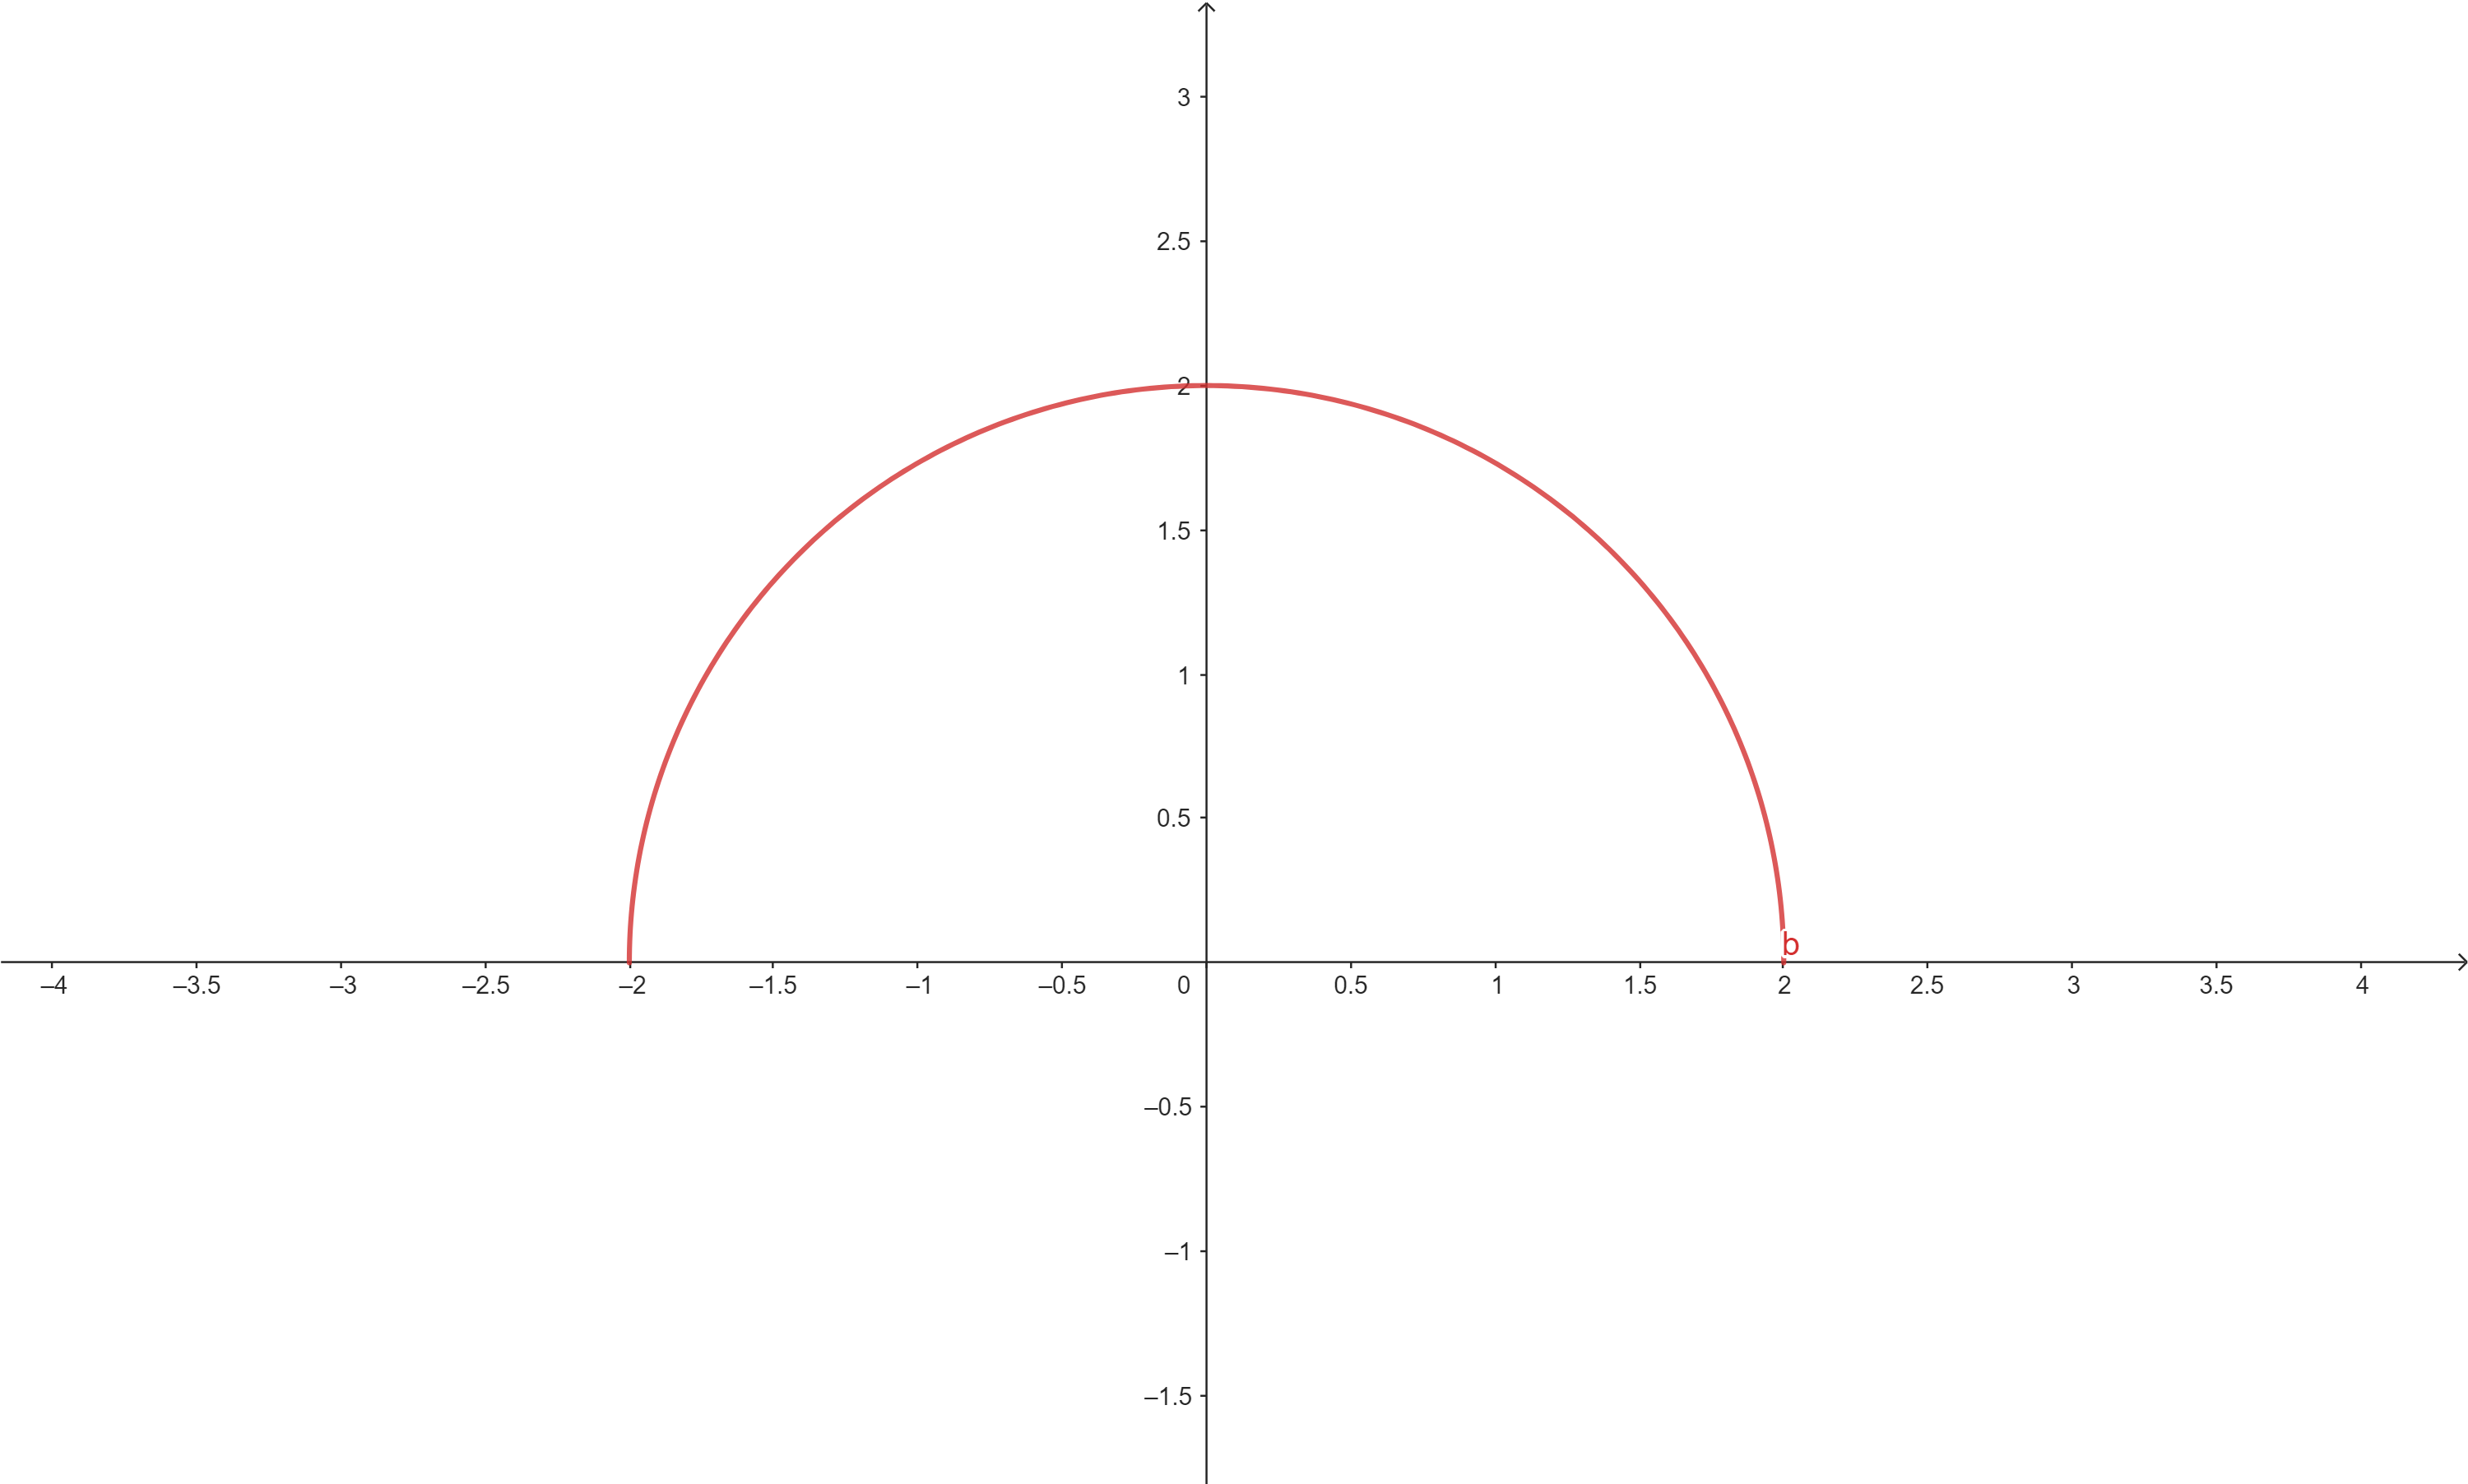
\includegraphics[width=\textwidth]{Capitoli/Capitolo1/sostegno_circ1.png}
        \caption{Sostegno di $\varphi(t)$ con $R=2$ e $t\in[0, \pi]$}
    \end{minipage}
    \hspace{1cm}
    \begin{minipage}{0.25\textwidth}
        \centering
        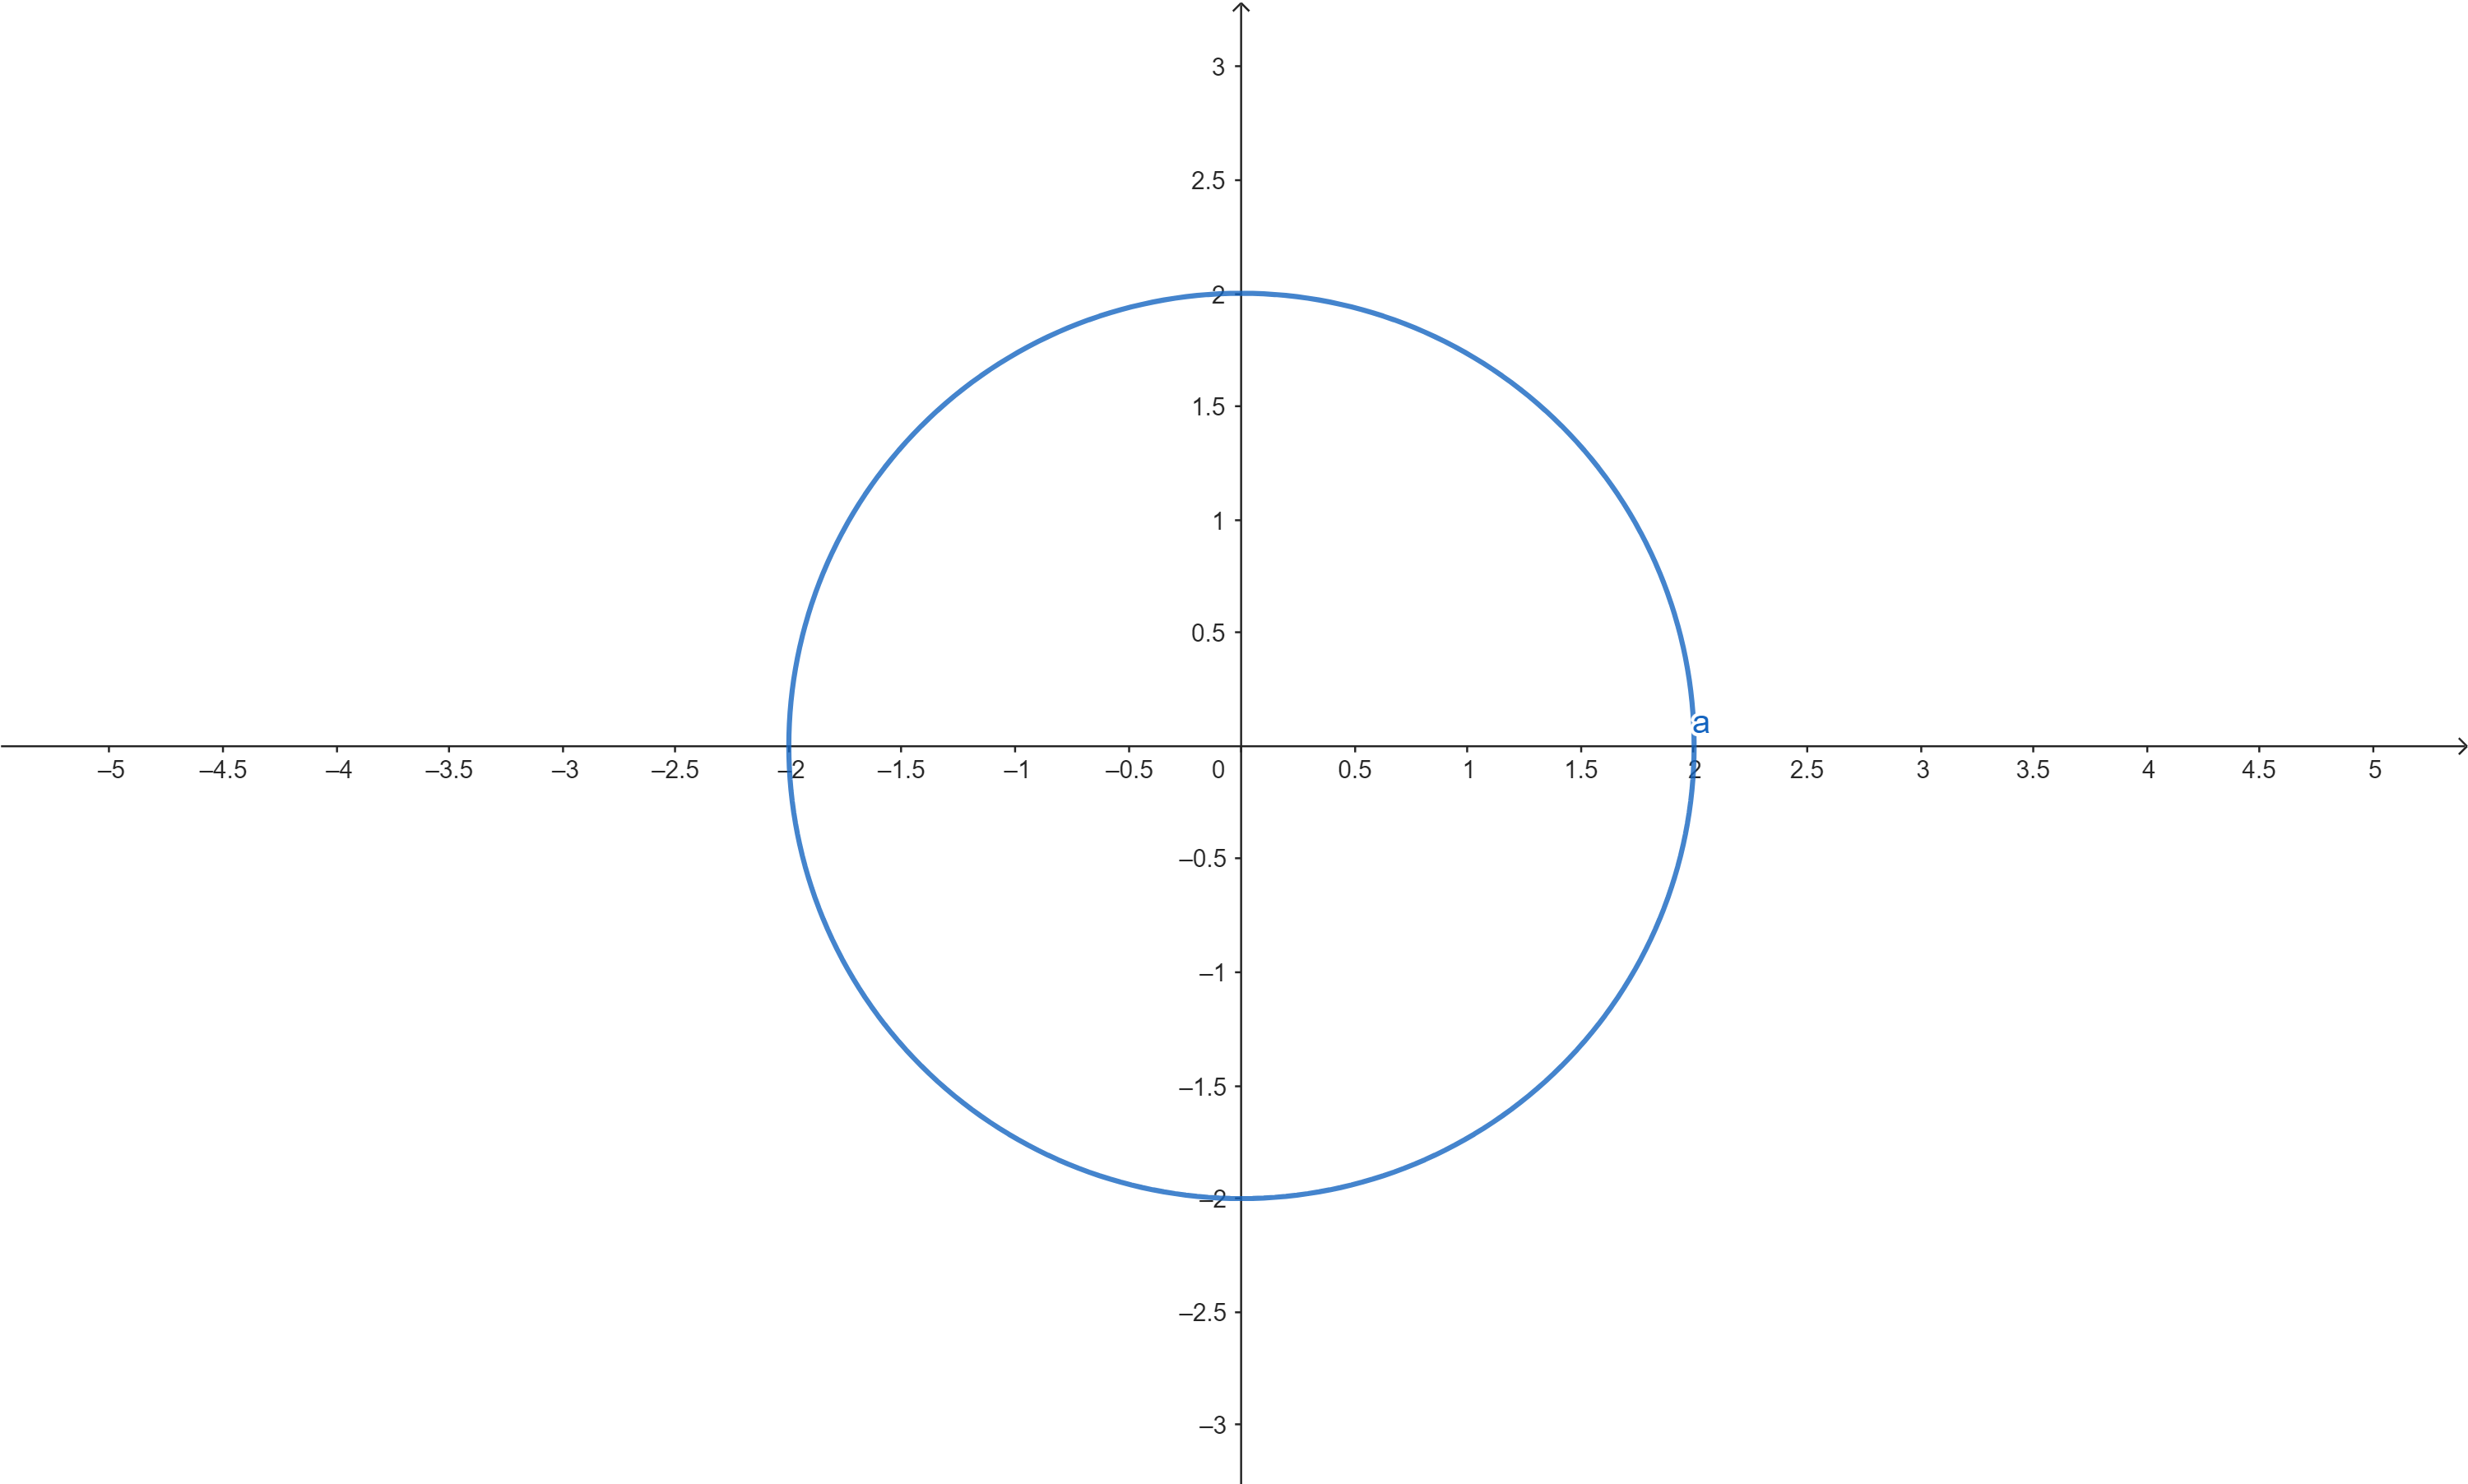
\includegraphics[width=\textwidth]{Capitoli/Capitolo1/sostegno_circ2.png}
        \caption{Sostegno di $\varphi(t)$ con $R=2$ e $t\in[0, 2\pi]$}
    \end{minipage}
    \hspace{1cm}
    \begin{minipage}{0.25\textwidth}
        \centering
        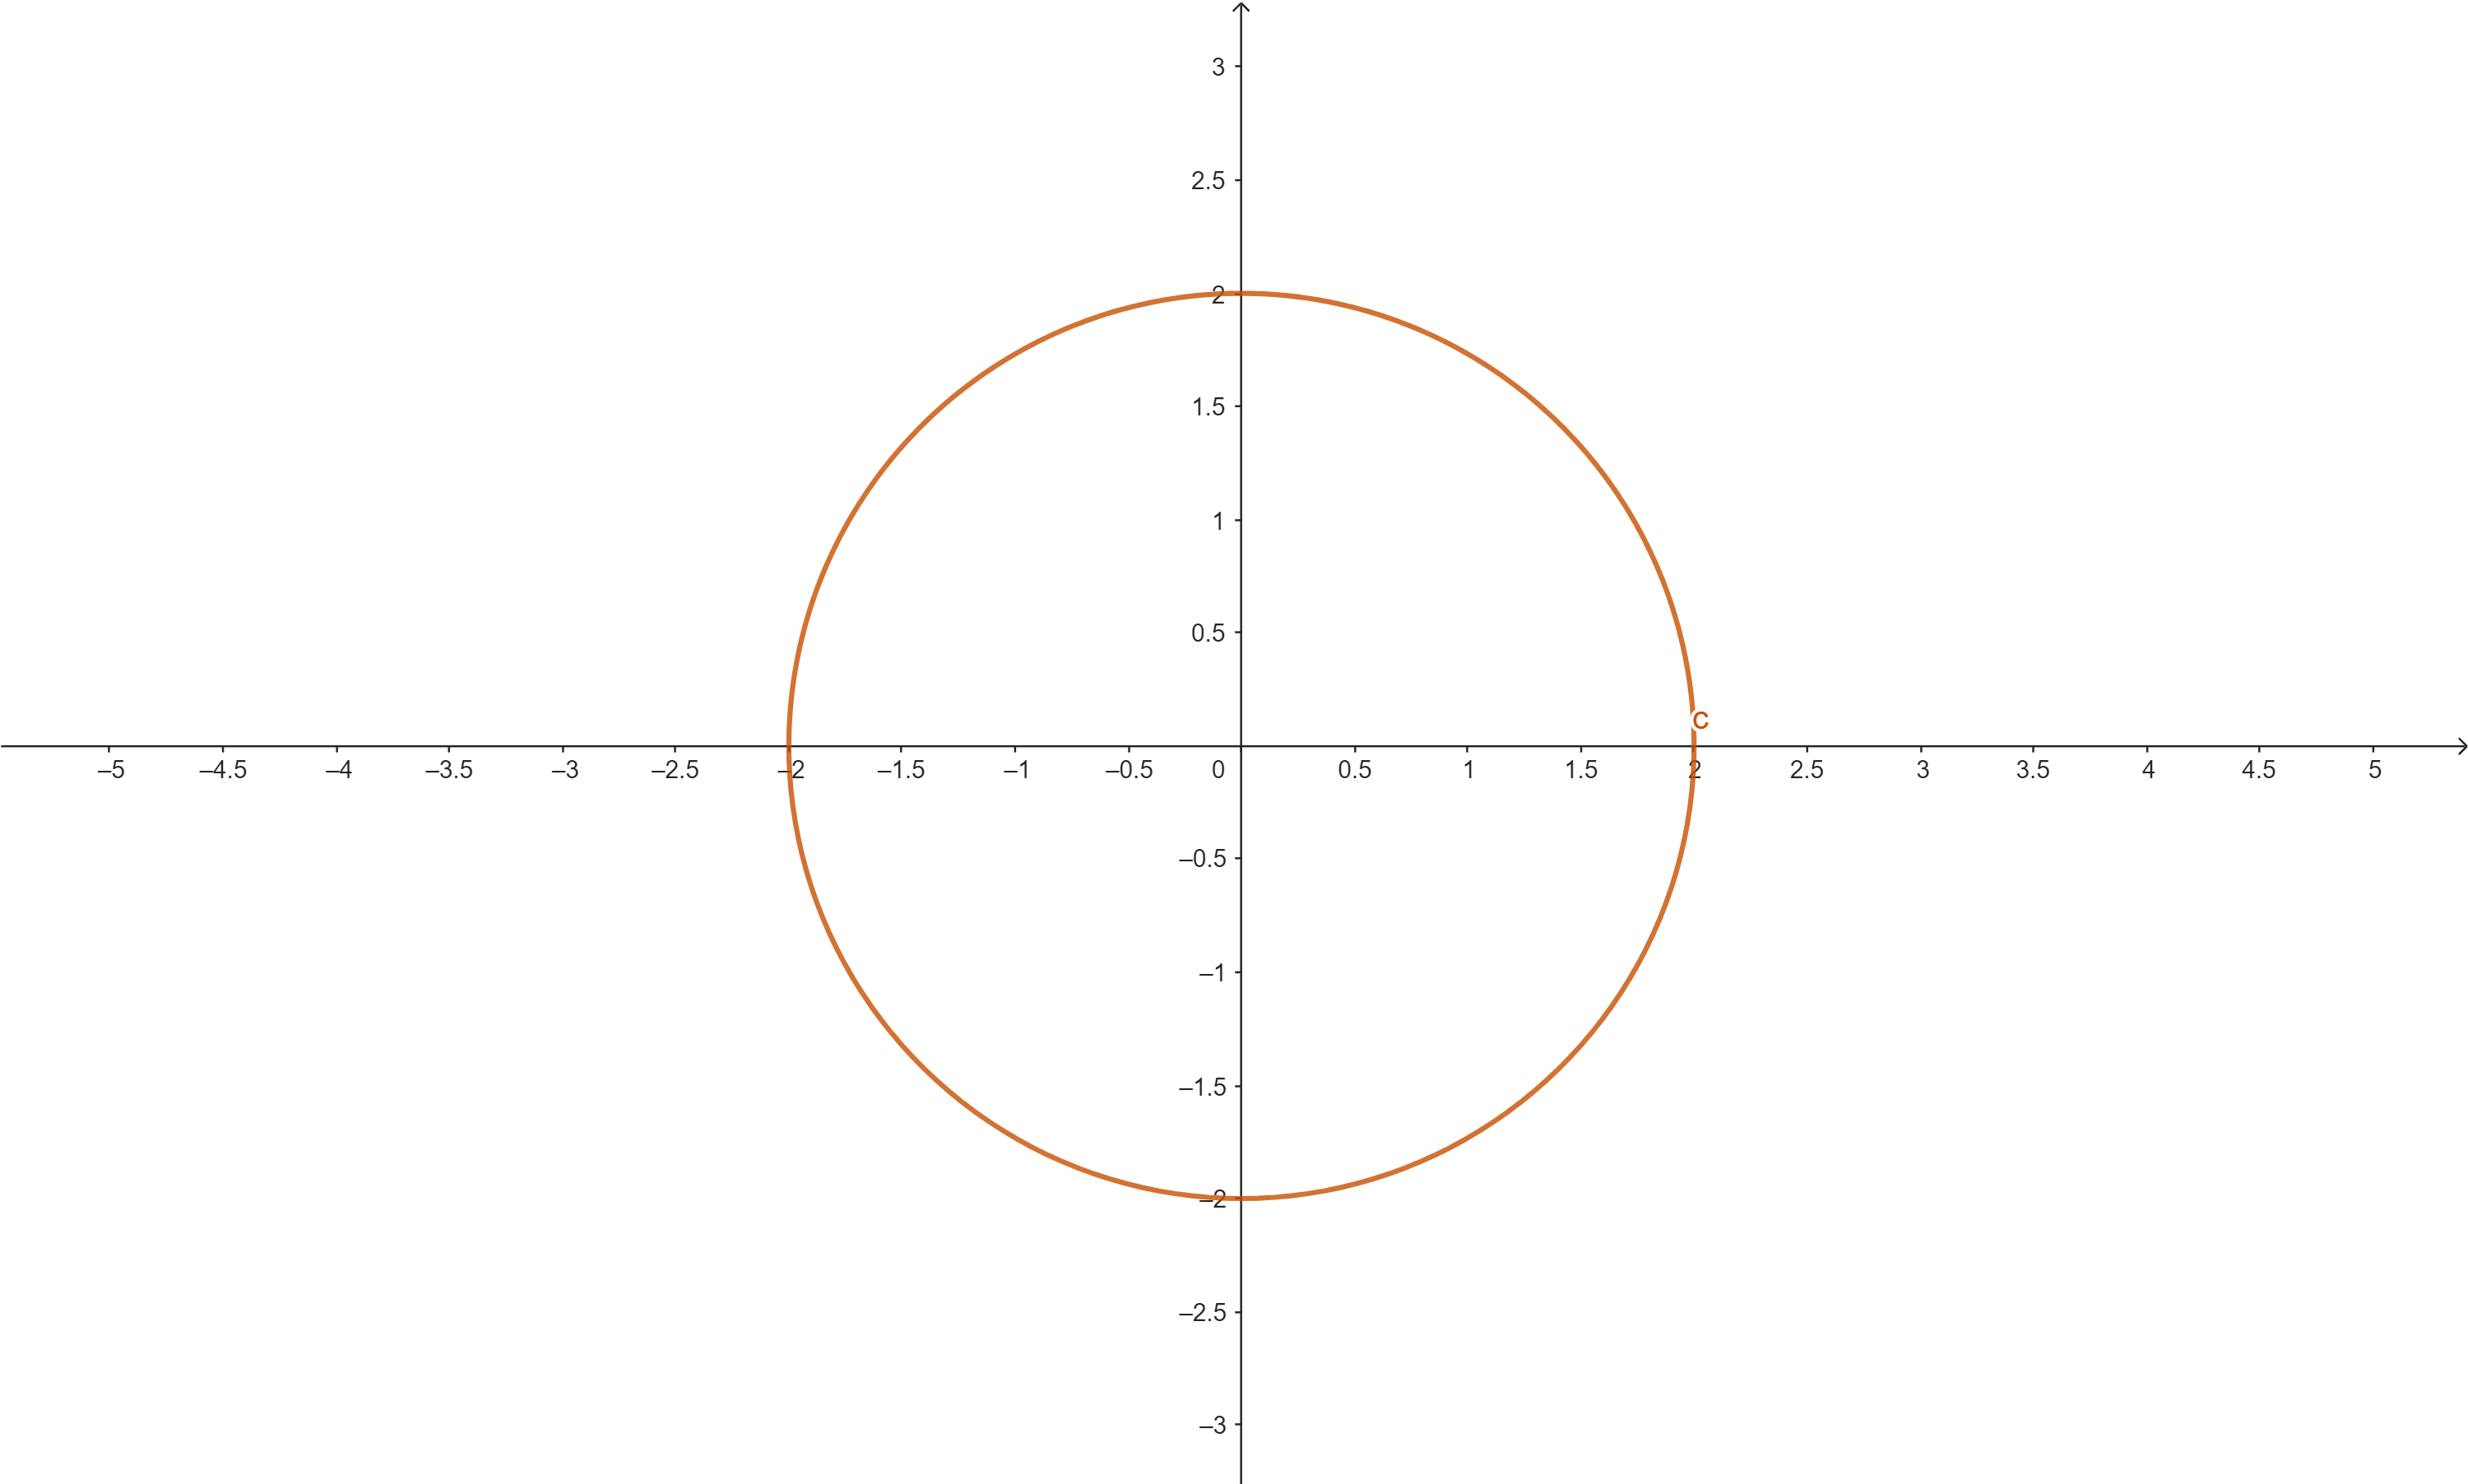
\includegraphics[width=\textwidth]{Capitoli/Capitolo1/sostegno_circ3.png}
        \caption{Sostegno di $\varphi(t)$ con $R=2$ e $t\in[0, 3\pi]$}
    \end{minipage}
\end{figure}
\end{example}
Da ciò si può osservare come, \textit{in primis}, la definizione di $I$ sia fondamentale nel tracciare il sostegno e, \textit{in secundis}, come, d'altra parte, il sostegno non identifichi la curva. A tal proposito infatti occorre notare che, benché le curve associate ai sostegni delle figure 1.2 e 1.3 siano diverse, i loro sostegni sono uguali.
\begin{example}    
    Un'altra casistica è quella rappresentata dalla curva di equazione $\varphi(t)=(R \cos(-t), R \sin(-t))$. Il suo sostegno, infatti, rimane la circonferenza (o l'arco) di raggio $R$, percorso tuttavia in senso orario.
\end{example}
\begin{definition}
    Sia $\varphi:[I \to \mathbb{R}^n]$ una curva parametrica. Allora si dice che $P_1=\varphi(t_1)$ \textbf{precede} $P_2=\varphi(t_2)$ nel verso delle $t$ crescenti se $t_1<t_2$ con $t_1, t_2 \in I$.
\end{definition}
\subsection{Proprietà delle curve parametriche}
Fatte tali premesse, si passi ad analizzare alcune proprietà delle curve.
\begin{definition}
    Una curva $\varphi:[a,b]\to\mathbb{R}^n$ si dice \textbf{chiusa} se $\varphi(a)=\varphi(b)$.
\end{definition}
\begin{oss}
    Si noti a tal proposito che la curva in figura 1.3 non è chiusa, mentre quella in figura 1.2 sì.
\end{oss}
\begin{definition}
    Una curva $\varphi:[a,b] \to \mathbb{R}^n$ si dice \textbf{semplice} se, $\forall$ $ t_1, t_2 \in [a,b]$ distinti di cui almeno uno \textit{interno} all'intervallo, risulta $\varphi(t_1)\neq\varphi(t_2)$.
\end{definition}
    \begin{oss}
        In altre parole, affinché $\varphi$ sia semplice, essa non deve autointersecarsi, se non, al più, negli estremi.
    \end{oss}
    \begin{oss}
        La curva in figura 1.2 è semplice.
    \end{oss}
\begin{definition}
    Una curva $\varphi:[a,b] \to \mathbb{R}^n$ si dice \textbf{regolare} se l'applicazione $\varphi$ è di classe $C^1$ in $[a,b]$ e se, $\forall t \in (a,b)$ il vettore $\varphi'(t)$ è diverso dal vettore nullo.
\end{definition}
A fronte di ciò, è possibile osservare che, se una curva è regolare, presi due valori distinti del parametro $t$, come $t_0, t_1$, è possibile tracciare la retta passante per $\varphi(t_0), \varphi(t_1)$. Allora, per $t_1 \to t_0$ si ottiene la \textbf{retta tangente} alla curva $\varphi$ in $\varphi(t_0)$.
Si definisce allora $\varphi'(t_0)=(\varphi_1'(t_0), \dots, \varphi_n'(t_0))$ \textbf{vettore tangente} alla curva $\varphi$ in $\varphi(t_0)$.
\begin{definition}
    Se $\varphi$ è regolare, si definisce \textbf{versore tangente} il normalizzato del vettore tangente a $\varphi$ in $\varphi(t_0)$, ovvero:
    \begin{equation}
        T(t_0)=\frac{\varphi'(t_0)}{|\varphi'(t_0)|}
    \end{equation}
\end{definition}
    \begin{oss}
        Data questa informazione, può diventare utile valutare direttamente $|\varphi'(t)|$ per stabilire la regolarità di una curva. Tale quantità è talvolta definita \textbf{velocità scalare}.
    \end{oss}
    \begin{oss}
        Una curva regolare è priva di cuspidi o punti angolosi.
    \end{oss}
\begin{example}
    Si valuti ora la seguente curva: $\varphi(t)=(t^3, t^2)$ con $t \in [-1, 1]$.
    Rispetto alle proprietà elencate, si può affermare che:
    \begin{itemize} 
        \item non è chiusa perché $\varphi(-1)=(-1,1)\neq(1,1)=\varphi(1)$;
        \item è semplice perché se fosse $\varphi(t_1) = \varphi(t_2)$, allora si avrebbe:
$
\begin{cases}
    t_1^3 = t_2^3 \\
    t_1^2 = t_2^2
\end{cases}
$
\\Ciò però significa che $t_1=t_2$.
    \item non è regolare poiché la sua derivata $\varphi(t)=(3t^2, 2t)$ si annulla in entrambe le componenti per $t=0$.
    \end{itemize}
Può essere utile visualizzare tale curva riscrivendone le equazioni in forma cartesiana. Si ricava dalla prima componente che $x=t^3 \iff t=x^\frac{1}{3}$. Allora, sostituendo nella seconda componente, $y=t^2 \iff y=\left(x^\frac{1}{3}\right)^2 \iff y=x^\frac{2}{3}$. Il grafico di tale funzione mostra, per l'appunto, la presenza di una cuspide in $t=0$, come già osservato in precedenza.\\
Tuttavia si può anche osservare che la curva può essere vista come l'unione di due curve regolari $\varphi_+$ nel semiasse positivo e $\varphi_-$ nel semiasse positivo negativo.
\end{example}
\begin{definition}
    Una curva $\varphi:[a,b]\to\mathbb{R}^n$ si dice \textbf{regolare a tratti} se esiste una suddivisione di $[a,b]$ in un numero \textit{finito} di intervalli $[t_i, t_{i+1}]$ in cui $\varphi$ sia regolare.
\end{definition}
\subsubsection{Curve cartesiane}
    Si studino ora le cosiddette curve \textbf{cartesiane}, definite come: 
    \begin{equation}
        y=f(x) \text{ con } x \in [a,b] 
    \end{equation}
    cioè, in forma parametrica,
    \begin{equation}
        \begin{cases}
            x=t \text{ con } t\in[a,b]\\ y=f(t)
        \end{cases}\\
    \end{equation}
    Di esse si può osservare che se, $f \in C^1$ allora la curva è regolare. Inoltre le curve cartesiane sono sempre semplici, giacché $t$ è iniettiva, e non sono mai chiuse.

\subsubsection{Curve in coordinate polari}
    Altre curve da analizzare sono le curve \textbf{in forma polare} ovvero del tipo:
    \begin{equation}
        \varrho=\varrho(\theta) 
    \end{equation}
    oppure in forma parametrica come 
    \begin{equation}
        \begin{cases}
            x=\varrho(\theta)\cos(\theta)\\
            y=\varrho(\theta)\sin(\theta)
        \end{cases}
    \end{equation}
    con $(x,y) \in \mathbb{R}\setminus \left\{(0,0)\right\}$, $\varrho \in \left[0, +\infty\right]$ e $\theta \in \left[0, 2\pi\right]$.\\
    Tale specifica rispetto alle caratteristiche della curva serve a sottolineare il fatto che una curva che si annulli in un qualche punto a causa di $\varrho=0$ e $\theta$ conseguentemente non definito, non sia regolare.\\
    Si noti che nel caso di una circonferenza il raggio $\varrho(t)=\text{cost}$.\\
    Il tangente in questo caso è
    \begin{equation}
        (x'(\theta), y'(\theta))=(\varrho'(\theta)\cos(\theta)-\varrho(\theta)\sin(\theta), \text{ } \varrho'(\theta)\sin(\theta)+\varrho(\theta)\cos(\theta))
    \end{equation}
    Dunque la norma della curva è:
    \begin{equation}
        |(x'(\theta), y'(\theta))|=\sqrt{\varrho'^2(\theta)+\varrho^2(\theta)}
    \end{equation} 
    Ne consegue che, se la curva non ha zeri doppi in $\left(\theta_1, \theta_2\right)$, allora è regolare in $\left[\theta_1, \theta_2\right]$.\\
    Si prenda ora il caso specifico in cui $\varphi$ è una curva in coordinate polari e $[a,b] \subseteq [0, 2\pi]$.
    Per quanto riguarda la proprietà di chiusura della curva, si presentano due scenari: 
    \begin{itemize}
        \item Se $[\theta_0, \theta_1] \subsetneq [0, 2\pi]$ allora la curva è chiusa per $\varrho(\theta_0)=\varrho(\theta_1)=0$;
        \item Se $[\theta_0, \theta_1]=[0, 2\pi]$ allora la curva è chiusa per $\varrho(0)=\varrho(2\pi)$
    \end{itemize}
    Rispetto alla proprietà di semplicità, si osserva:
    \begin{itemize}
        \item Se $[\theta_0, \theta_1] \subseteq [0, 2\pi]$ allora la curva è semplice se $\nexists$ $\theta_i, \theta_j \in (0,2\pi)$ tali che $\varrho(\theta_i)=\varrho(\theta_j)=0$
    \end{itemize}
\newpage
\section{Curve equivalenti}
\begin{definition}
    Due curve $\varphi: I\to \mathbb{R}^n$ e $\psi:J\to \mathbb{R}^n$ si dicono \textbf{equivalenti} se $\exists$ $\eta:I\to J$ di classe $C^1(I)$ suriettiva e tale che $\eta'(t) \neq 0$ $\forall$ $t \in I$ per cui si abbia
    \begin{equation}
        \varphi(t)=\psi(\eta(t)) \text{ } \forall \text{ } t \in I
    \end{equation}
\end{definition}
\begin{oss}
    $\eta$ è detta \textbf{cambio di parametro ammissibile}. 
\end{oss}
\begin{oss}
    Volendo studiare il segno delle curve, si ottiene:
    \begin{equation*}
        \varphi'(t)=\psi'(\eta(t))\eta'(t)
    \end{equation*}
    Si noti che $\eta'$ non turba la regolarità della curva poiché mantiene il proprio segno e non si annulla mai (per costruzione).
\end{oss}
\begin{oss}
    $\eta$ è per sua costruzione suriettiva e monotona, dunque è anche iniettiva. Pertanto $\eta$ è biunivoca e invertibile. Sfruttando $\eta^{-1}(s)$ si ottiene:
    \begin{equation}
        \psi(s)=\varphi(\eta^{-1}(s))
    \end{equation}
\end{oss}
\begin{oss}
    Se $\varphi$ e $\psi$ sono equivalenti come descritto, allora
    \begin{equation}
        \varphi\sim\psi
    \end{equation}
    Si tratta proprio di una relazione di equivalenza dal momento che:
    \begin{equation}
        \text{Per } \eta(t)=t \text{, } \varphi(t)=\varphi(\eta(t))=\varphi(t), \text{ cioè } \varphi\sim\varphi
    \end{equation}
    Il risultato dell'osservazione precedente mostra che se $\varphi\sim\psi$ allora $\psi\sim\varphi$.
    Infine, prese $\varphi$, $\psi$, $\chi$ tali che $\varphi\sim\psi$ e $\psi\sim\chi$ allora:
    $\varphi=\psi(\eta(t))$ e $\psi(t)=\chi(\zeta(t))$. Allora
    \begin{equation}
        \varphi(t)=\psi(\eta(t))=\chi(\zeta(\eta(t))) \text{ cioè } \varphi\sim\chi
    \end{equation}
\end{oss}
\begin{definition}
    L'applicazione $\eta$ che permette di passare dalla rappresentazione parametrica di $\varphi$ a quella di $\psi$ è detta anche \textbf{$C^1$ diffeomorfismo}.
\end{definition}
\begin{definition}
    Date due curve equivalenti $\varphi$ e $\psi$, si dice che $\psi$ è la riparametrizzazione di $\varphi$.
\end{definition}
Si può osservare che due curve equivalenti hanno lo stesso sostegno. Tuttavia tale condizione non è sufficiente siccome per l'equivalenza è necessario che il sostegno sia percorso nel medesimo numero di volte.\\
La nozione di equivalenza può essere rafforzata, come segue.
\begin{definition}
    Due curve equivalenti come sopra si dicono \textbf{equvalenti con lo stesso verso} se il loro sostegno è percorso nello stesso verso, cioè se: $\eta'>0$
\end{definition}
\section{Lunghezza di una curva}
Si consideri una curva continua $\varphi:[a,b] \to \mathbb{R}^n$ definita su un intervallo chiuso e limitato $[a,b]$. È possibile associare ad ogni \textit{partizione} 
\begin{equation}
    a=t_0<t_1<...<t_N=b
\end{equation}
la poligonale $\mathcal{P}$ inscritta nella curva e di vertici $\varphi(a),\varphi(t_1),\dots,\varphi(t_{N-1}), \varphi(b)$. La lunghezza di tale poligonale sarà pari a:
\begin{equation}
    \ell(\mathcal{P})=\sum\limits_{i=1}^{N}{|\varphi(t_i)-\varphi(t_{i-1})}
\end{equation}
Tale valore è un'approssimazione della lunghezza effettiva della curva per difetto, il cui errore diminuisce in maniera proporzionale al numero di segmenti che compongono la poligonale.
\begin{figure}[H]
    \centering
    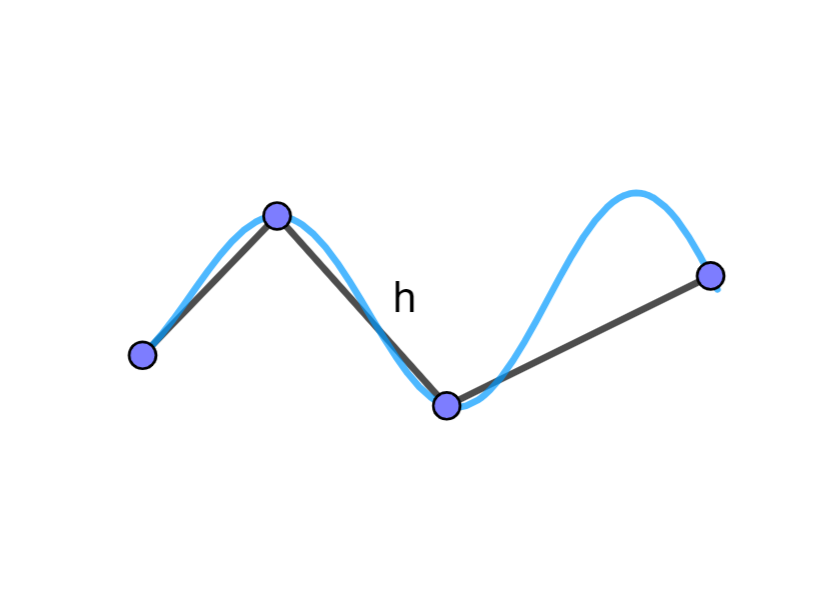
\includegraphics[width=0.33\textwidth]{Capitoli/Capitolo1/lunghezza1.png}
    \hspace{0.05\textwidth} % Spazio tra le immagini
    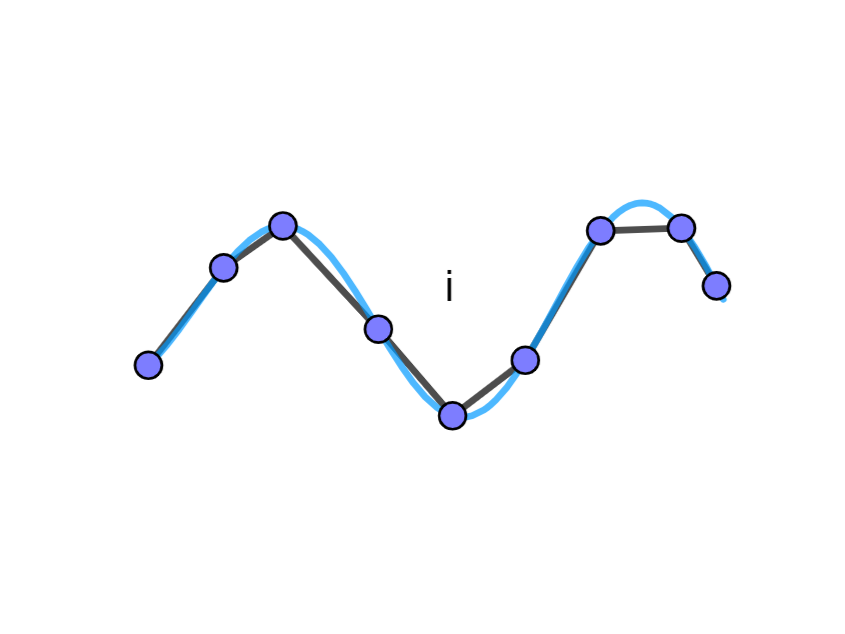
\includegraphics[width=0.33\textwidth]{Capitoli/Capitolo1/lunghezza2.png}
    \caption{In figura la stessa curva la cui lunghezza viene misurata con poligonali diverse.}
\end{figure}
\begin{definition}
    Sia $\varphi:[a,b]\to \mathbb{R}^n$, allora si dice \textbf{lunghezza di un arco di curva} continua la quantità
    \begin{equation}
        L(\varphi)=\sup\limits_{l}(\mathcal{P})
    \end{equation}
    dove $\mathcal{P} \in \Pi$ con $\Pi=\left\{\text{poligonali inscritte nella curva}\right\}$.
\end{definition}
\begin{definition}
    Si dice che una curva $\varphi: [a,b] \to \mathbb{R}^n$ è \textbf{rettificabile} se 
    \begin{equation}
        \sup\limits_{\mathcal{P}\in\Pi}L(\varphi)<+\infty
    \end{equation}
\end{definition}
\begin{theorem}[Teorema di rettificabilità]
Sia $\varphi: [a,b] \to \mathbb{R}^n$ una curva di classe $C^1$. Allora essa è rettificabile e 
\begin{equation}
    L(\varphi)=\int_{a}^{b}{|\varphi'(t)|dt}
\end{equation}
\end{theorem}
\begin{oss}
    La lunghezza di una curva $C^1$ è invariante per riparametrizzazione.
\end{oss}
\begin{oss}
    Si osservi che vale: $\ell(\mathcal{P})\leq \int_{a}^{b}{|\varphi'(t)|dt}$. Infatti:
    \begin{equation}
        \begin{aligned}
            \ell(\mathcal{P}) &= \sum\limits_{i=1}^{N} \left| \varphi(t_i) - \varphi(t_{i-1}) \right|= \sum\limits_{i=1}^{N} \left\lvert \int_{t_{i-1}}^{t_i} \varphi'(t) \, dt \right\rvert \\
            &\leq \sum\limits_{i=1}^{N} \int_{t_{i-1}}^{t_i} \left\lvert \varphi'(t) \right\rvert \, dt = \int_{a}^{b} \left\lvert \varphi'(t) \right\rvert \, dt
        \end{aligned}
    \end{equation}
\end{oss}
\begin{example}
    Detta 
    \begin{equation*}
        f(x)= \begin{cases}
            0 \text{ se } x=0\\ x\sin(\frac{1}{x}) \text{ se } x\neq 0
        \end{cases}
    \end{equation*}
    allora una curva non rettificabile può essere 
    \begin{equation*}
        \varphi(t)=(t, f(t)) \text{ con } t\in[0,1]
    \end{equation*}
\end{example}
\section{Triedro di Frénet}
Si desideri ora sviluppare un sistema di riferimento intrinseco ad una curva $\varphi:[a, b] \to \mathbb{R}^n$ regolare e tale che $\varphi'(t)$ ed il versore tangente $T$ siano ben definiti su $(a, b)$.
\begin{definition}
    Si definisce l'\textbf{ascissa curvilinea} o parametro d'arco $s=s(t)$ come
    \begin{equation}
        s(t)=\int_a^t{\left\lvert \varphi'(\tau) \right\rvert d\tau}
    \end{equation}
    \end{definition}
    \begin{oss}
        $s:[a,b] \to [0, L(\varphi)=L]$ è una parametrizzazione della curva regolare $\varphi$. Inoltre, $s'(t)=|\varphi'(t)| \neq 0$ su $(a,b)$.
    \end{oss} 
    \begin{oss}
        Riparametrizzando $\varphi$ con ascissa curvilinea $s=s(t)$, si può dire che $\varphi\sim\psi$. Dunque, rinominata $t(s)=s^{-1}(t)$, vale $\psi(s)=\varphi(t(s))$. Derivando la riparametrizzazione, si ha che:
        \begin{equation}
            \psi'(s)=\varphi'(t(s)) \text{ } t'(s) \overset{\substack{\text{Derivata}\\\text{ inversa}}}{=} \frac{\varphi'(t(s))}{s'(t)} = \frac{\varphi'(t(s))}{|\varphi'(t(s))|}
        \end{equation}
        Ciò mostra come il vettore tangente a $\psi$ sia in ogni punto un versore tangente $T(s)$
    \end{oss}

\paragraph*{Prodotto scalare in $\mathbb{R}^n$}
Siano $\underline{v}=(v_1, \dots, v_n)$ e $\underline{w}=(w_1, \dots, w_n)$ vettori di $\mathbb{R}^n$. Allora
\begin{equation}
    \langle \underline{v}, \underline{w} \rangle = \sum\limits_{i=1}^{n}{v_iw_i} 
\end{equation}
\paragraph*{Prodotto vettoriale in $\mathbb{R}^3$}
Siano $\underline{v}=(v_1, v_2, v_3)$ e $\underline{w}=(w_1, w_2, w_3)$ vettori di $\mathbb{R}^3$. Allora
\begin{equation}
    \underline{v} \wedge \underline{w}=
    \left\lvert\begin{matrix}
         e_1 & e_2 & e_3 \\
               v_1 & v_2 & v_3 \\
               w_1 & w_2 & w_3
            \end{matrix}\right\rvert
\end{equation}
\begin{lemma}
    Siano $u, v$ definiti in $I\to\mathbb{R}^3$ e derivabili. Allora:
    \begin{align}
        \frac{d}{dt}{\langle u(t), v(t) \rangle} = \langle u'(t), v(t) \rangle + \langle u(t), v'(t) \rangle \\
        \frac{d}{dt}\left(u(t) \wedge v(t)\right) = u'(t) \wedge v(t) + u(t) \wedge v'(t)
    \end{align}
\end{lemma}
\begin{proposition}
    Sia $w:I\to\mathbb{R}^3$ derivabile e tale che $\exists$ $c>0$ per cui $|w(t)|=c$ $\forall$ $t \in I$. Allora $w'(t) \perp w(t)$.
\end{proposition}
    \begin{proof}
        Affinché i due vettori siano ortogonali, occorre che il loro prodotto scalare sia nullo. Pertanto, poiché per ipotesi $|w(t)|=c$
        \begin{equation}
            |w(t)|^2=c^2 \iff \langle w(t), w(t) \rangle = c
        \end{equation}
        Derivando rispetto a $t$ e applicando l'equazione 1.26, si ha che:
        \begin{equation}
            \frac{d}{dt}{\langle w(t), w(t)\rangle}\overset{\substack{\text{Prop.} \\ \text{prod. scal.} }}{=}2 \langle w'(t), w(t) \rangle = \frac{d c^2}{dt}=0
        \end{equation}
    \end{proof}
\begin{oss}
    La curva $\psi:[c,d] \to \mathbb{R}^3$ parametrizzata con ascissa curvilinea è tale che $|\psi'(s)|=1$. Di conseguenza, per la proposizione, $\psi''(s) \perp \psi'(s)$ e, nella fattispecie, $T'(s) \perp T (s)$.  
\end{oss}
\begin{definition}
    Sia $\psi$ una riparametrizzazione di $\varphi$ biregolare nel suo intervallo di parametrizzazione, cioè sia tale che $\psi \in C^2([c,d])$ e $\psi''(s) \neq 0$ $forall$ $s \in [c,d]$. Allora si può definire il \textbf{versore normale} il normalizzato della derivata del versore tangente. Quindi:
    \begin{equation}
        N(s)=\frac{\psi''(s)}{|\psi''(s)|}=\frac{T'(s)}{|T'(s)|}
    \end{equation}
\end{definition}
\begin{definition}
    Si dice \textbf{curvatura} di $\psi$ in $\psi(s)$ 
    \begin{equation}
        k(s)= |\psi''(s)|
    \end{equation}
\end{definition}
\begin{definition}
    Si dice \textbf{piano osculatore} per $\psi$ in $\psi(s)$ il piano generato da 
    \begin{equation}
        \left\{T(s), N(s)\right\}
    \end{equation} 
\end{definition}
È appena stato definito un nuovo versore $N$ linearmente indipendente. È possibile ottenere una base ortonormale di $\mathbb{R}^3$ attraverso il prodotto esterno dei due versori.
\begin{definition}
    Si dice \textbf{versore binormale} il versore:
    \begin{equation}
        B(s)=T(s) \wedge N(s)
    \end{equation}
\end{definition}
\begin{definition}
    Si dice \textbf{piano normale} per $\psi$ in $\psi(s)$ il piano generato da
    \begin{equation}
        \left\{N(s), B(s)\right\}
    \end{equation}
\end{definition}
\newpage
\begin{definition}
    Si dice \textbf{piano rettificato} per $\psi$ in $\psi(s)$ il piano generato da
    \begin{equation}
        \left\{ B(s), T(s) \right\}
    \end{equation}
\end{definition}
\begin{definition}
    Si dice \textbf{triedro di Frénet} o \textbf{terna intrinseca} la base ortonormale di $\mathbb{R}^3$ positivamente orientata formata da
    \begin{equation}
        \left\{T(s), N(s), B(s)\right\}
    \end{equation}
\end{definition}
\begin{theorem}[Formule di Frénet]
    Sia $\varphi: I \to \mathbb{R}^3$ una curva biregolare, di classe $C^3(I)$ e parametrizzata con ascissa curvilinea. Allora, $\exists!$ $k:I\to \mathbb{R}_+$, $\tau:I\to\mathbb{R}$ tali che:
    \begin{equation}
        \begin{cases}
            T'(s)=k(s)N(s)\\
            N'(s)=-k(s)T(s)-\tau(s)B(s)\\
            B'(s)=\tau(s)N(s)
        \end{cases}
    \end{equation}
    \end{theorem}
    \begin{proof}
        Si parta dalla prima equazione: 
        \begin{equation}
            T'(s)=k(s)N(s).        
        \end{equation}
        Tale risultato discende dalla definizione stessa di $T'$. Si consideri infatti che $T'(s)\perp T(s)$ poiché $|T(s)|=1$ $\forall$ $s$. Prendendo poi $k(s)=|T'(s)|$, si ottiene l'identità tra i due membri.\\
        Si analizzi poi la terza equazione:
        \begin{equation}
            B'(s)=\tau(s)N(s)
        \end{equation}
        Per definizione di $B$, esso discende dal prodotto vettoriale degli altri due versori. Se ne studi la derivata:
        \begin{equation}
            B'(s)=T'(s)\wedge N(s) + T(s) \wedge N(s) \overset{\substack{T'(s)\parallel N(s)}}{=} T(s)\wedge N'(s)
        \end{equation}
        Quindi, poiché $B'(s)\perp T(s)$ e $B'(s) \perp B(s)$, allora $B'(s) \parallel N(s)$. Definendo $\tau(s)=|B'(s)|$, l'equazione è soddisfatta.\\
        Infine, si affronti la seconda equazione:
        \begin{equation}
            N'(s)= -k(s)T(s)- \tau(s)B(s)
        \end{equation}
        Siccome $\left\{T(s), N(s), B(s)\right\}$ è positivamente orientata,
        \begin{equation}
            N(s)=B(s) \wedge T(s)
        \end{equation}
        Derivando $N$, si ha che
        \begin{equation}
            \begin{aligned}
                N'(s)&=B'(s)\wedge T(s) + B(s) \wedge T'(s)=\\
                &\overset{\substack{\text{Frénet}}}{=} \tau(s)N(s)\wedge T(s) + B(s) \wedge k(s)N(s)\\
                &\overset{\substack{N \wedge T = -B\\B \wedge N =-T}}{=} -\tau(s)B(s)- k(s)T(s)
            \end{aligned}
        \end{equation}
    \end{proof}
\begin{oss}
    Risolvendo il sistema di equazioni differenziali, si potrebbe mostrare come valga anche l'implicazione inversa.
\end{oss}
\begin{oss}
    Poiché $B(s)$ è ortogonale al piano osculatore, si può notare che se esso ha derivata nulla, il piano rimane costante.
\end{oss}
\begin{definition}
    Si dice \textbf{torsione} di $\varphi$ in $\varphi(s)$
    \begin{equation}
        \tau(s)=|B'(s)|
    \end{equation}
\end{definition}
\begin{definition}
    Una curva si dice \textbf{piana} se la sua torsione è nulla, cioè se essa giace su un piano.
\end{definition}
\begin{definition}
    Si dice \textbf{cerchio osculatore} per una curva $\varphi:[a,b]\to \mathbb{R}^3$ biregolare, il cerchio giacente nel piano osculatore, avente raggio $r=\frac{1}{k(t)}$ con $k(t)$ curvatura di $\varphi(t)$ e centro sul semiasse normale a $\varphi(t)$.
\end{definition}
\begin{definition}
    Il raggio del cerchio osculatore è detto \textbf{raggio osculatore}.
\end{definition}
Nel corso dell'ultimo capitolo si è cercato di trovare una parametrizzazione di una curva in $\mathbb{R}^3$ ed è stata proposta l'ascissa curvilinea, il cui calcolo non è però sempre comodo.\\
Pertanto è possibile osservare che se una generica $\psi:[a,b]\to \mathbb{R}^3$ è una curva riparametrizzata con parametro qualunque, allora valgono su di essa le formule di Frénet generalizzate.
\begin{theorem}[Formule di Frénet generalizzate]
    Sia $\psi$ una curva riparametrizzata con parametro qualunque su cui valgano le ipotesi del Teorema 2. Allora vale:
    \begin{equation}
        \begin{cases}
            T'(t)=|\psi'(t)| k(t) N(t)\\
            N'(t)=-|\psi'(t)| k(t) T(t) - |\psi'(t)| \tau(t)B(t)\\
            B'(t)=|\psi'(t)|\tau(t)N(t)
        \end{cases}
    \end{equation}
    Dove:
    \begin{align}
        &T(t)=\frac{\psi'(t)}{|\psi'(t)|}\\
        &N(t)=\frac{T'(t)}{|T'(t)|}\\
        &B(t)=\frac{\psi'(t)\wedge \psi''(t)}{|\psi'(t)\wedge \psi''(t)|}\\
        &k(t)=\frac{|\psi'(t)\wedge\psi''(t)|}{|\psi'(t)|^3}\\
        &\tau(t)=\frac{\langle\psi'(t)\wedge \psi''(t), \psi'''(t)\rangle}{|\psi'(t)\wedge \psi''(t)|^2}
    \end{align}    
\end{theorem}
\section{Integrale curvilineo}
\begin{definition}
    Sia $\gamma$ una curva regolare e $\varphi:[a,b]\to \mathbb{R}^n$ una sua rappresentazione parametrica. Sia poi $f:A\subseteq \mathbb{R}^n \to \mathbb{R}$ una funzione in più variabili tale che $\varphi([a,b])\subseteq A$ e $f \circ\varphi$ sia continua su $[a,b]$.\\
    Allora si può definire l'\textbf{integrale curvilineo di prima specie} di f su $\gamma$
    \begin{equation}
        \int_\gamma{fds} := \int_{a}^{b}{f(\varphi(t))|\varphi'(t)|dt}
    \end{equation}
\end{definition}
\begin{theorem}[Invarianza per equivalenza di curve]
    L'integrale curvilineo di prima specie è invariante per equivalenza di curve.
\end{theorem}
    \begin{proof}
        Si ricordino innanzitutto le ipotesi:\\
        \indent $\varphi:[a,b]\to \mathbb{R}^n$ regolare, parametrizzazione di $\gamma$.\\
        \indent $f:A\subseteq\mathbb{R}^n \to \mathbb{R}$ con $\varphi([a,b]) \subseteq A$\\
        \indent $\psi:[c, d]\to \mathbb{R}^n$ regolare, parametrizzazione di $\hat{\gamma}$ e $\varphi \sim \psi$.\\
        La tesi da mostrare è:
        \begin{equation}
            \int_\gamma{f ds}=\int_{\hat{\gamma}}{f ds}
        \end{equation}
        Per definizione dell'integrale curvilineo di prima specie si ha:
        \begin{equation}
            \int_\gamma{fds}= \int_{a}^{b}{f(\varphi(t))|\varphi'(t)|dt}
        \end{equation}
        Ponendo, $s=\eta(t)$ si ha che
        \begin{equation}
            \varphi(t)=\psi(\eta(t)) \iff \varphi(\eta^{-1}(s))=\psi(s)    
        \end{equation}
        e
        \begin{equation}
            \psi'(s)=\varphi'(\eta^{-1}(s))(\eta^{-1})'(s)
        \end{equation}
        Perciò, risolvendo l'integrale con la seguente sostituzione 
        \begin{equation}
            \begin{aligned}
            &s=\eta(t) \\ &t=\eta^{-1}(s) \\ &dt=(\eta^{-1})'(s)ds
            \end{aligned}
        \end{equation}
        si ha che
        \begin{equation}
            \begin{aligned}
                &\int_\gamma{fds} = \int_{a}^{b}{f(\varphi(t))\ |\varphi'(t)|\ dt}\\
                &\overset{\text{sub}}{=} \int_{\eta(a)}^{\eta(b)}{f(\varphi(\eta^{-1}(s)))\ |\varphi(\eta^{-1}(s))|\ (\eta^{-1})'(s)\ ds}
            \end{aligned}
        \end{equation}
        Ora, dipendentemente dalla monotonia di $\eta$ si avrà:\\
        \indent$\eta^{-1}>0 \Rightarrow \ \eta(a)=c,\  \eta(b)=d,\  (\eta^{-1})'(s)>0$
        \begin{equation}
            \begin{aligned}
                &\int_{\eta(a)}^{\eta(b)}{f(\varphi(\eta^{-1}(s)))\ |\varphi'(\eta^{-1}(s))| \ (\eta^{-1})'(s)\ ds}=\\
                &\int_{c}^{d}{f(\psi(s))\ |\psi'(s)| \ ds}= \int_{\hat{\gamma}}{f \ ds}
            \end{aligned}
        \end{equation}
        \indent$\eta^{-1}<0 \Rightarrow \eta(a)=d, \ \eta(b)=c, \ (\eta^{-1})'(s)<0$
        \begin{equation}
            \begin{aligned}
                &\int_{\eta(a)}^{\eta(b)}{f(\varphi(\eta^{-1}(s)))\ |\varphi'(\eta^{-1}(s))| \ (\eta^{-1})'(s)\ ds}=\\
                &\int_{d}^{c}{f(\psi(s))\ (-|\psi'(s)|)\ ds} = \int_{c}^{d}{f(\psi(s))\ |\psi'(s)|\ ds}= \int_{\hat{\gamma}}{f\ ds}
            \end{aligned}
        \end{equation}
    \end{proof}
    \begin{oss}
        La distinzione finale discende dal fatto che, presa l'equazione 1.55 e applicatovi il modulo, se $\eta$ è crescente, si ha
        \begin{equation}
            \begin{aligned}
                |\psi'(s)|&=|\varphi'(\eta^{-1}(s))(\eta^{-1})'(s)|\overset{\substack{\text{Prop.}\\\text{Norma}}}{=}|(\eta^{-1})(s)|\ |\varphi'(\eta^{-1}(s))=\\
                &\overset{\eta'>0}{=} (\eta^{-1})'(s)\ |\varphi'(\eta^{-1})(s)|
            \end{aligned}
        \end{equation}
        se $\eta$ è decrescente,
        \begin{equation}
            \begin{aligned}
                |\psi'(s)|&=|\varphi'(\eta^{-1}(s))(\eta^{-1})'(s)|\overset{\substack{\text{Prop.}\\\text{Norma}}}{=}|(\eta^{-1})(s)|\ |\varphi'(\eta^{-1}(s))=\\
                &\overset{\eta'<0}{=} -(\eta^{-1})'(s)\ |\varphi'(\eta^{-1})(s)|
            \end{aligned}
        \end{equation}
    \end{oss}
\begin{corollary}
    La lunghezza di una curva regolare a tratti è invariante per equivalenza.
    \end{corollary}
    \begin{proof}
        La dimostrazione del corollario discende dalla dimostrazione precedente, in cui $f \equiv 1$.
        Infatti si avrebbe:
        \begin{equation}
            L(\varphi)=\int_{a}^{b}{|\varphi'(t)|\ dt}=\int_{c}^{d}{|\psi'(s)|\ ds}=L(\psi)
        \end{equation}
    \end{proof}
    \begin{oss}
        Sia $\varphi$ una parametrizzazione della curva $\gamma$ mediante ascissa curvilinea. Allora,
        \begin{equation}
            \int_{\gamma}{f \ ds}= \int_{0}^{L}{f(\varphi(t))|\varphi'(t)|\ dt} \overset{\substack{|\varphi'(t)| \equiv 1\\ \text{per param.}}}{=} \int_{0}^{L}{f(\varphi(t))\ dt}
        \end{equation}
        è proprio l'area sottesa da $f\Big|_{\gamma}$
    \end{oss}